\section{Transformée de Fourier}
Ce qu'on a vu jusqu'à maintenant fonctionne pour des fonctions périodiques, mais qu'arrive-t-il lorsqu'on tente d'étendre cela à des fonctions qui ne le sont pas? En d'autres mots, pour une fonction qui a une période infinie (donc qui n'est pas périodique), comment se comportent nos précédentes trouvailles? Alors, on regarde les précédentes équations dans la limite où $T \rightarrow \infty$. On commence par recopier (2.5) et (2.6) en changeant les bornes d'intégration pour (2.6), ce qu'on peut faire par (1.4).

\begin{equation}
    f(x) = \sum_{n = -\infty}^{\infty}c_ne^{2\pi inx/T} \ \text{ où } \ c_n = \frac{1}{T}\int_{-T/2}^{T/2}f(x)e^{-2\pi inx/T}dx
\end{equation}

Soit $\omega_n = \frac{2\pi n}{T}$ la fréquence angulaire pour un $n$ donné. Alors, la différence entre deux $\omega_n$ successifs est $\Delta \omega_n = \frac{2\pi}{T}\Delta n = \frac{2\pi}{T}$ puisque l'écart entre deux $n$ successifs est évidemment de 1. Dans la limite où $T \rightarrow \infty$, $\Delta \omega_n$ est infinitésimale et $\omega_n$ devient essentiellement une variable continue $\omega$. Sachant cela, on effectue quelques manipulations sur l'équation (3.1). D'abord, pour une fonction de période finie,

\begin{equation*}
    f(x) = \sum_{n = -\infty}^{\infty}c_ne^{2\pi inx/T} \cdot 1 = \sum_{n = -\infty}^{\infty}c_ne^{i\omega_nx} \Delta n = \sum_{n = -\infty}^{\infty}\left(c_n\frac{T}{2\pi}\right)e^{i\omega_nx}\Delta \omega_n  
\end{equation*}

Puis, dans la limite où la fonction a en fait une période infinie, on a 

\begin{equation*}
    f(x) = \lim_{T\rightarrow\infty}\sum_{n = -\infty}^{\infty}\left(c_n\frac{T}{2\pi}\right)e^{i\omega_nx}\Delta \omega_n = \lim_{T\rightarrow\infty}\sum_{n = -\infty}^{\infty}\left(\frac{1}{2\pi}\int_{-T/2}^{T/2}f(x)e^{-i\omega_nx}dx\right) e^{i\omega_nx}\Delta \omega_n
\end{equation*}
\begin{equation}
    = \int_{-\infty}^{\infty}\left(\frac{1}{2\pi}\int_{-\infty}^{\infty}f(x)e^{-i\omega x}dx\right)e^{i\omega x}d\omega = \int_{-\infty}^{\infty}c(\omega)e^{i\omega x}d\omega 
\end{equation}

où on pose 

\begin{equation}
    c(\omega) = \frac{1}{2\pi}\int_{-\infty}^{\infty}f(x)e^{-i\omega x}dx
\end{equation}

Comme auparavant, $c(\omega)$ est un coefficient (en général complexe) qui nous dit "combien" il y a de $e^{i\omega x}$ dans $f(x)$. En fait, l'équation (3.3) va être ce qu'on appelle la transformée de Fourier (TF) de $f(x)$ et permet de décrire la "quantité" de chaque fréquence $\omega$ dans $f(x)$. Ainsi, la TF permet de décomposer $f(x)$ en ses fréquences. D'un autre côté, (3.2) correspond à la transformée de Fourier inverse (TFI), parce qu'elle permet depuis les fréquences connues $c(\omega)$ de reconstruire $f(x)$. C'est l'opération inverse de la TF, d'où son nom.

Par ailleurs, bien que la TF soit à la base pour les fonctions qui ne sont pas périodiques, elle s'applique tout de même aux fonctions périodiques. En effet, on a déjà dit que $4\pi$ ou $6\pi$ (des multiples de la "plus petite période" $2\pi$) peuvent aussi être des périodes de $\sin(x)$. En poussant ce raisonnement à l'extrême, on peut dire que la période de $\sin(x)$ est infinie. Cela peut être dit pour n'importe quelle fonction périodique et il va de soi que (3.2) et (3.3) s'appliquent aussi aux fonctions périodiques.

Finalement, selon les démarches de (3.2), le facteur $\frac{1}{2\pi}$ aurait pu être déplacé à l'extérieur de la somme si on le voulait. Dans ce cas, on aurait ce facteur devant (3.2) et il n'y aurait plus rien devant (3.3). En fait, ce choix dépend des auteurs mais rien ne change mathématiquement. Certains séparent même le facteur pour mettre $\frac{1}{\sqrt{2\pi}}$ devant (3.2) et (3.3). C'est purement esthétique.

\subsection{Exemple : Pulse rectangulaire}
Soit un pulse rectangulaire de hauteur 1 défini comme 

\begin{equation*}
    \text{Rect}(x) = \begin{cases}
        1 & \text{si } \abs{x} < \tau/2 \\
        0 & \text{sinon}
    \end{cases}
\end{equation*}

\begin{figure}[H]
    \centering
        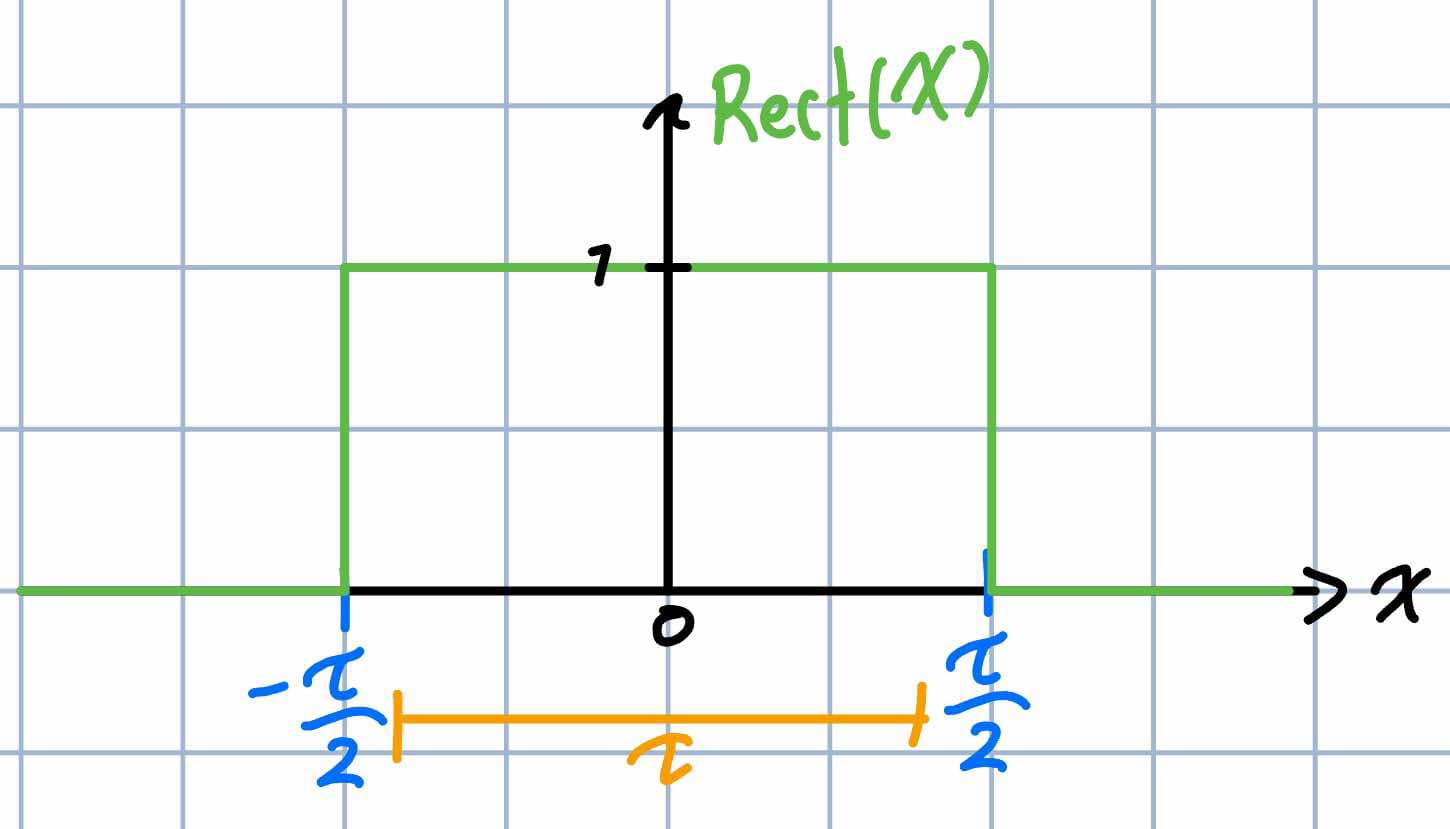
\includegraphics[width=0.3\textwidth]{images/ch3/pulse_rectangulaire.jpg}
    \caption{Pulse rectangulaire de hauteur 1}
    \end{figure}

Par (3.3), 

\begin{equation*}
    c(\omega) = \frac{1}{2\pi}\int_{-\infty}^{\infty}\text{Rect}(x)e^{-i\omega x}dx = \frac{1}{2\pi}\int_{-\tau/2}^{\tau/2}e^{-i\omega x}dx = \frac{1}{2\pi}\int_{-\tau/2}^{\tau/2}\left(\cos(\omega x) - i\sin(\omega x)\right)dx
\end{equation*}
\begin{equation*}
    = \frac{1}{2\pi}\left[\int_{-\tau/2}^{\tau/2}\underbrace{\cos(\omega x)}_\text{paire}dx - i\int_{-\tau/2}^{\tau/2}\underbrace{\sin(\omega x)}_\text{impaire}dx\right] = \frac{1}{\pi}\int_{0}^{\tau/2}\cos(\omega x)dx = \frac{1}{\pi \omega}\sin(\frac{\tau\omega}{2})
\end{equation*}

Si on pose $\tau = 1$ à des fins de représentation, on peut voir de quoi à l'air $c(\omega)$ dans cet exemple.

\begin{figure}[H]
    \centering
        
\includegraphics[width=0.6\textwidth]{images/ch3/coeff_pulse_rectangulaire.png}
    \caption{$c(\omega)$ pour le pulse rectangulaire ($\tau = 1$)}
    \end{figure}

Par (3.2),

\begin{equation*}
    \text{Rect}(x) = \int_{-\infty}^{\infty}\frac{\sin(\frac{\tau\omega}{2})}{\pi \omega}e^{i\omega x}d\omega
\end{equation*}

Pour vérifier que cela tient, il faudrait évaluer l'intégrale, ce qui à priori ne semble pas simple du tout. En utilisant la formule d'Euler, on trouve

\begin{equation*}
    \text{Rect}(x) = \int_{-\infty}^{\infty}\frac{\sin(\frac{\tau\omega}{2})}{\pi \omega}\left(\cos(\omega x) + i\sin(\omega x)\right)d\omega = \int_{-\infty}^{\infty}\frac{\sin(\frac{\tau\omega}{2})}{\pi \omega}\cos(\omega x)d\omega + i\int_{-\infty}^{\infty}\frac{\sin(\frac{\tau\omega}{2})}{\pi \omega}\sin(\omega x)d\omega
\end{equation*}

Par rapport à $\omega$, l'intégrande de la première intégrale est paire alors que celle de la deuxième intégrale est impaire. Ainsi, la deuxième est nulle et on se retrouve avec 

\begin{equation*}
    \text{Rect}(x) = \int_{-\infty}^{\infty}\frac{\sin(\frac{\tau\omega}{2})}{\pi \omega}\cos(\omega x)d\omega
\end{equation*}

Malgré les simplifications, calculer cette dernière intégrale ne semble pas facile. On peut l'approximer, par exemple, en prenant des bornes d'intégration $\left[a, b\right]$ qui tendent progressivement vers $(-\infty, \infty)$. Les figures ci-dessous présentent cette approximation avec différentes bornes d'intégration pour le pulse rectangulaire où $\tau = 1$. Naturellement, on voit que plus les bornes tendent vers $(-\infty, \infty)$, plus on se rapproche du vrai pulse rectangulaire.

\begin{figure}[H]
    \centering
        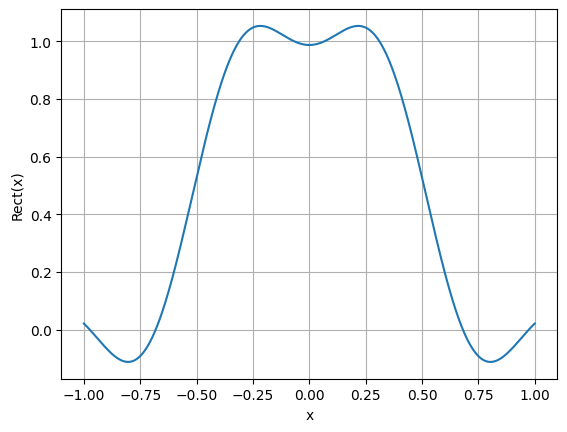
\includegraphics[width=0.45\textwidth]{images/ch3/bornes_10.png}
        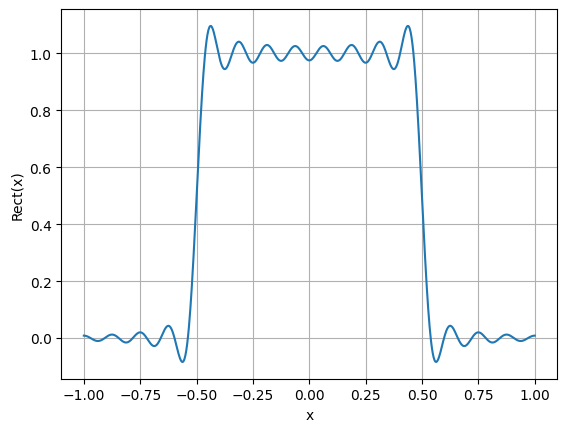
\includegraphics[width=0.45\textwidth]{images/ch3/bornes_50.png}
    \caption{TFI de Rect$(x)$ ($\tau=1$) avec bornes $[-10, 10]$ (à gauche) et $[-50, 50]$ (à droite)}
    \end{figure}

    \begin{figure}[H]
        \centering
            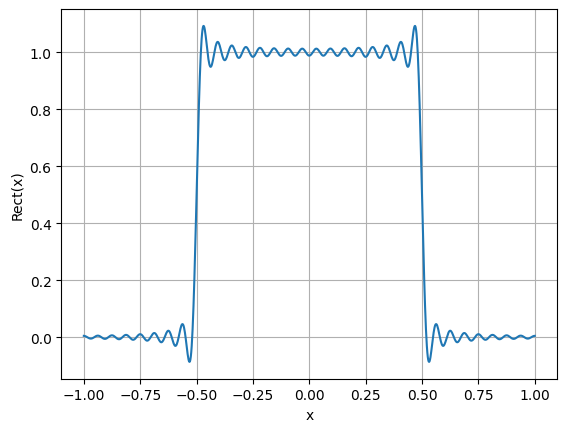
\includegraphics[width=0.45\textwidth]{images/ch3/bornes_100.png}
            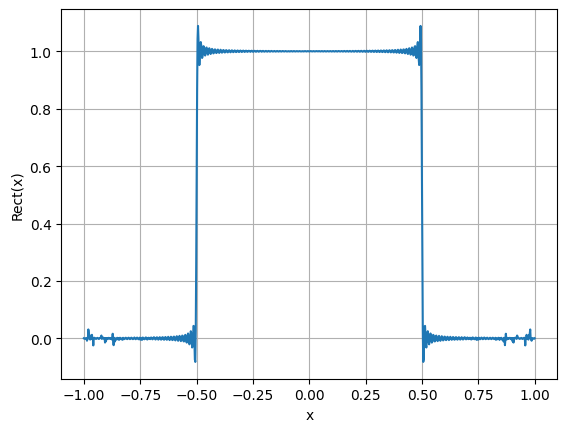
\includegraphics[width=0.45\textwidth]{images/ch3/bornes_500.png}
        \caption{TFI de Rect$(x)$ ($\tau=1$) avec bornes $[-100, 100]$ (à gauche) et $[-500, 500]$ (à droite)}
        \end{figure}